\documentclass[openany,b5paper]{article}

%-----------------Preamble-----------------
\usepackage{amsmath}
\usepackage{amsfonts}
\usepackage{pgfplots}

%-----------------Title-----------------
\title{Empirical Research in Management and Economics\\Formula Sheet}

%-----------------Document-----------------
\begin{document}
\maketitle

\section{Descriptive Statistics}
\subsection{Measure of Location}
\subsubsection{Mean}
\begin{align}
\bar{x} = \dfrac{1}{n} \displaystyle\sum_{i=1}^{n} x_i
\end{align}
\subsubsection{Median}
For odd number of elements in a dataset:
\begin{align}
\tilde{x} = x_{\frac{n+1}{2}}
\end{align}
For even number of elements in a dataset:
\begin{align}
\tilde{x} = \dfrac{x_{\frac{n}{2}}+x_{\left(\frac{n}{2}+1\right)}}{2}
\end{align}
\subsubsection{Mode}
\begin{align}
Mo(x) = \max(f(x_i))
\end{align}

\subsubsection{Quartile}
Measure of percentage of elements less than or equal to a term

\subsection{Measure of Spread}
\subsubsection{Variance}
Variance measured on the whole population
\begin{align}
\sigma^2 = \dfrac{1}{n} \sum_{i=1}^{n} \left( x_i - \bar{x} \right)^2
\end{align}
\subsubsection{Sample Variance}
Variance measured on a sample population
\begin{align}
s^2 = \dfrac{1}{n-1} \sum_{i=1}^{n} \left( x_i - \bar{x} \right)^2
\end{align}

\subsubsection{Standard Deviation and Sample Standard}
\begin{align}
\sigma = \sqrt{\sigma^2}\\
s=\sqrt{s^2}
\end{align}

\subsubsection{Co-efficient of Variance}
\begin{align}
v = \dfrac{s}{\bar{x}}
\end{align}

\subsection{Skewness}
\subsubsection{Types of Skewness}
\begin{table}[!h]
\centering
\begin{tabular}{c|c|c}
Name & Other Name & Characteristic\\
\hline
Right Skew & Positive Skew & Data concentrated on the lower side\\
Symmetric Distribution & Normal Distribution & Data distributed evenly\\
Left Skew & Negative Skew & Data concentrated on the higher side
\end{tabular}
\end{table}

\subsubsection{Measure of Skewness}
Skewness is measured by the Moment Co-efficient of Skewness.
\begin{align}
g_m &= \dfrac{m_3}{s^3}, \text{ where}\\
m_3 &= \dfrac{1}{n}\sum_{i=1}^{n} \left( x_i - \bar{x} \right)^3
\end{align}

\paragraph{Type of Skewness}
The type of skewness from the value is $g_m$ is:
\begin{table}[h!]
\centering
\begin{tabular}{c|c}
Value of $g_m$ & Type\\
\hline
$g_m = 0$ & Symmetric\\
$g_m > 0$ & Positive Skew\\
$g_m < 0$ & Negative Skew
\end{tabular}
\end{table}

\paragraph{Degree of Skewness}
The degree of skewness from the value is $g_m$ is:
\begin{table}[h!]
\centering
\begin{tabular}{c|c}
Value of $g_m$ & Degree\\
\hline
$|g_m| > 1$ & High Skewness\\
$0.5 <|g_m| \geq 1$ & Moderate Skewness\\
$|g_m| \leq 0.5$ & Low Skewness
\end{tabular}
\end{table}

\subsection{Kurtosis}
Kurtosis is the measure of peakedness of data. Fisher's kurtosis measure is defined as:
\begin{align}
\gamma &= \dfrac{m_4}{s^4}, \text{ where}\\
m_4 &= \dfrac{1}{n}\sum_{i=1}^{n} \left( x_i - \bar{x} \right)^4
\end{align}

\subsubsection{Type of Kurtosis}
The types of kurtosis from the value of $\gamma$ are:
\begin{table}[h!]
\centering
\begin{tabular}{c|c}
Value of $\gamma$ & Type\\
\hline
$\gamma = 0$ & Normal Distribution or Mesokurtic\\
$\gamma < 0$ & Flattened or Platykurtic\\
$\gamma > 0$ & Peaked or Lepokurtic
\end{tabular}
\end{table}

\section{Hypothesis Testing}
\subsection{T-Test}
\begin{align}
T = \dfrac{\bar{X}-\mu}{\frac{s}{\sqrt{n}}}
\end{align}
where:
\begin{align*}
\bar{X} &= \text{Sample Mean}\\
\mu &= \text{Assumed Mean}\\
s &= \text{Number of Samples}\\
n &= \text{Number of observations}
\end{align*}

If $T < t_c$ the $H_0$ is not rejected. $t_c$ is a functions of level of significance $(\alpha)$ and degrees of freedom $(v = n -1)$.

\subsection{$\chi^2$ Test}
\begin{align}
\chi^2 = \sum_i \sum_j \dfrac{(h_{ij}^o-h_{ij}^e)^2}{h_{ij}^e}
\end{align}
where:
\begin{align*}
h_e &= \text{Expected Value}\\
h_o &= \text{Actual Value}
\end{align*}

If $\chi^2 < \chi_c^2$ then $H_0$ is not rejected. $\chi_c$ is a functions of level of significance $(\alpha)$ and degrees of freedom $(v = (i-1)(j-1))$.

\section{Research and Survey Design}
\subsection{Population Covariance}
\begin{align}
\text{Cov}(x,y)=\dfrac{1}{n} \sum_{i=1}^n (x_i-\mu_x)(y_i-\mu_y)
\end{align}
\subsection{Sample Covariance}
\begin{align}
\text{Cov}(x,y)=\dfrac{1}{n-1} \sum_{i=1}^n (x_i-\bar{x})(y_i-\bar{y})
\end{align}
\subsection{Bravais-Pearson Correlation Co-efficient}
\begin{align}
r &= \dfrac{\sum_{i=1}^n (x_i-\bar{x})(y_i-\bar{y})}{\sqrt{\sum_{i=1}^n (x_i-\bar{x})^2} \cdot \sqrt{\sum_{i=1}^n (y_i -\bar{y})^2}}\\
& = \dfrac{\text{Cov}(x,y)}{\sqrt{\text{Var}(x) \cdot \text{Var}(y)}}\\
& = \dfrac{\text{Cov}(x,y)}{\sigma_x \cdot \sigma_y}
\end{align}

\section{Estimation of Regression Function}
For the regression functions:
\begin{align}
	Y_i = \beta_0 + \beta_1 X_1\\
	\hat{Y_i} = \hat{\beta_0} + \hat{\beta_1} X_1\\
\end{align}
where $Y_i$ is the observed dependent variable (DV), $\hat{Y_i}$ is the estimated DV, and $X_i$ is the independent variable (IV).
\begin{align}
	u_i &= Y_i - \hat{Y_i}\\
	\Rightarrow Y_i &= \hat{Y_i} + u_i\\
	\Rightarrow Y_i &= \hat{\beta_0} + \hat{\beta_1} X_1 + u_i\\
	Y_i &= \beta_0 + \beta_1 X_i+\epsilon_i
\end{align}
The objective function is:
\begin{align*}
	\displaystyle^{\min}_{u_i} \sum u_i &= \min \sum_i \left[ Y_i - \hat{\beta_0} - \hat{\beta_1} X_i\right]^2\\
	&\text{Since the regression function passes through: } \left(\bar{X},\bar{Y}\right) \tag*{}\\
	\beta_0 &= \bar{Y} - \hat{\beta_1}\bar{X}\\
	\displaystyle^{\min}_{u_i} \sum u_i &= \min \sum_i \left[ Y_i - \bar{Y} + \hat{\beta_1} \bar{X} - \hat{\beta_1} X_i\right]^2\\
	& = \min \sum_i \left[\left(Y_i - \bar{Y}\right) - \hat{\beta_1} \left(X_i - \bar{X}\right)\right]^2\\
	& = \min \sum_i \left[\left(Y_i - \bar{Y}\right)^2 - 2 \cdot \left(Y_i - \bar{Y}\right) \cdot \hat{\beta_1} \left(X_i - \bar{X}\right) + \hat{\beta_1}^2 \left(X_i - \bar{X}\right)^2 \right]\\
	& = \min \left[\sum_i \left(Y_i - \bar{Y}\right)^2 - 2 \cdot \hat{\beta_1} \sum_i \left(Y_i - \bar{Y}\right) \cdot  \left(X_i - \bar{X}\right) + \hat{\beta_1}^2 \sum_i \left(X_i - \bar{X}\right)^2 \right]\\
	\Rightarrow u_i^{\beta_1} &= - 2 \sum_i \left(Y_i - \bar{Y}\right) + 2 \hat{\beta_1} \left(X_i - \bar{X}\right)^2 = 0 \tag{For optima Conditions}\\
	\Rightarrow \hat{\beta_1} &= \boxed{\dfrac{\sum_i (Y_i - \bar{Y})(X_i - \bar{X})}{\sum_i (X_i - \bar{X})^2}}\\
	\Rightarrow \hat{\beta_0} &= \boxed{\bar{Y} - \hat{\beta_1} \bar{X}}
\end{align*}

\subsection{Sum of Squares Error}
\begin{align}
	TSS &= \sum_i (Y_i - \bar{Y})^2\\
	& = \underbrace{\sum_i (\hat{Y_i}-\bar{Y})}_{\text{Explained Sum of Square Error (ESS)}} + \underbrace{\sum_i u_i^2}_{\text{Residual Sum of Squares Error (RSS)}}
\end{align}
\subsubsection{$R^2$: Coefficient of Determination}
\begin{align}
	R^2 &= \dfrac{\text{ESS}}{\text{TSS}}\\
	&= 1 - \dfrac{\text{RSS}}{\text{TSS}}\\
	&= 1 - \dfrac{\sum_i u_i^2}{\sum_i (Y_i-\bar{Y})^2}
\end{align}
For a regression analysis with single IV:
\begin{align*}
	\sqrt{R^2} = v
\end{align*}
\subsubsection{$\bar{R^2}$: Coefficient of Determination}
\begin{align}
	\bar{R^2}= 1 - \dfrac{\dfrac{\sum_i u_i^2}{(N-K-1)}}{\dfrac{\sum_i (Y_i-\bar{Y})^2}{(N-1)}}
\end{align}
where, $N$ is the number of observations and $K$ is the number of independent variables.

\subsection{T-Test}
Test for statistical significance of a single IV.
\begin{align}
	T = \dfrac{\hat{\beta_1}-0}{S_e(\hat{\beta_1})}
\end{align}
\subsection{F-Test}
Test for statistical significance of all IVs together.
\begin{align}
	F = \dfrac{\dfrac{\text{ESS}}{(K-1)}}{\dfrac{\text{RSS}}{(N-K)}} \tag{$F \geq F_c, H_0$ is rejected}
\end{align}

\subsection{Test for Heteroskedasticity}
\paragraph{Definition} $\sigma_{\epsilon_i} \forall  \epsilon_i \in [X_a, X_b] = \sigma_{\epsilon_i} \forall  \epsilon_i \in [X_{b+1}, X_c]$
\subsubsection{Durbin-Watson Test}
\begin{align}
	d_e = \dfrac{\sum_{t=2}^{n} (\hat{u_t}-\hat{u_{t-1}})^2}{\sum_{t=2}^{n} \hat{u_t}^2}
\end{align}
For the $H_0$: No autocorrelation:
\begin{table}[!h]
	\centering
	\begin{tabular}{l|c}
		$d$ & $H_0$\\
		\hline
		$0 \leq d_e \leq d_L$ \& $(4-d_L) \leq d_e \leq 4$ & Rejected\\
		$d_L < d_e \leq d_U$ \& $(4-d_U) < d_e \leq (4-d_L)$ & Decision Free Zone\\
		$d_L < d_e < D_U$ & Not rejected
	\end{tabular}
\end{table}

\section{Dummy Variables}
\subsection{Dummy Variable}
\begin{align}
	P_i = \beta_0 + \beta_1 S_1 + \beta_2 D_i + \epsilon_i\\
	E(P_i) =
		\begin{cases}
			(\hat{\beta_0}+\hat{\beta_2})+\hat{\beta_1}S_i, &D_i = 1\\
			\hat{\beta_0} + \hat{\beta_1}S_i, &D_i = 0
		\end{cases}
\end{align}

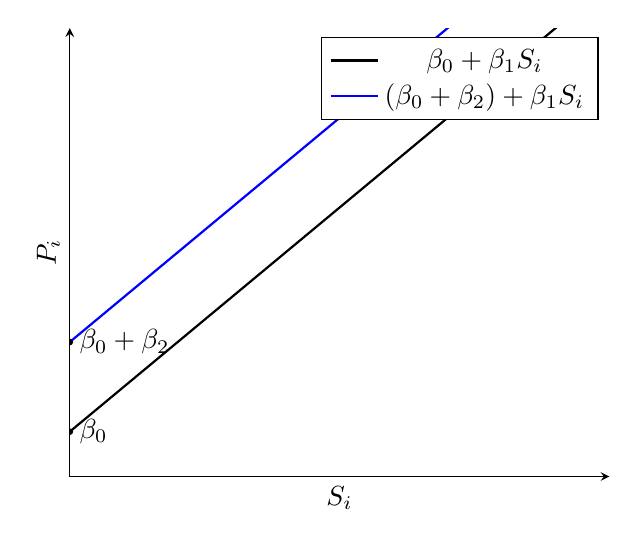
\begin{tikzpicture}
	\begin{axis}[axis lines = left, xmin = 0, ymin = 0, xmax = 10, ymax = 10, xlabel = $S_i$, ylabel = $P_i$, ticks=none]
		\addplot[domain=0:10,black, thick]{x+1};
		\addlegendentry{$\beta_0+\beta_1 S_i$}
		\addplot[domain=0:10,blue, thick]{x+3};
		\addlegendentry{$(\beta_0+\beta_2)+\beta_1 S_i$}
		\draw(axis cs:0,1)[fill]circle(1pt)node[right]{$\beta_0$};
		\draw(axis cs:0,3)[fill]circle(1pt)node[right]{$\beta_0+\beta_2$};
	\end{axis}
\end{tikzpicture}

\subsection{Slope Dummy Variable}
\begin{align}
	P_i = \beta_0 + \beta_1 S_1 + \beta_2 (S_i \cdot D_i) + \epsilon_i\\
E(P_i) =
\begin{cases}
	\hat{\beta_0} + \left(\hat{\beta_1}+\hat{\beta_2} \right)S_i, &D_i = 1\\
	\hat{\beta_0} + \hat{\beta_1}S_i, &D_i = 0
\end{cases}
\end{align}
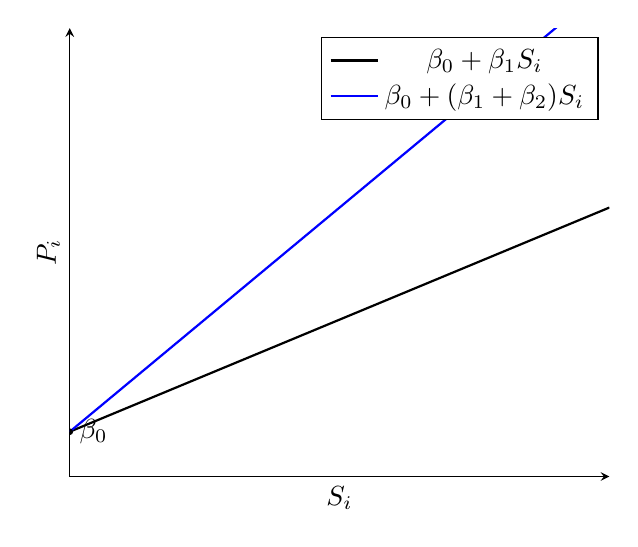
\begin{tikzpicture}
	\begin{axis}[axis lines = left, xmin = 0, ymin = 0, xmax = 10, ymax = 10, xlabel = $S_i$, ylabel = $P_i$, ticks=none]
		\addplot[domain=0:10,black, thick]{0.5 * x+1};
		\addlegendentry{$\beta_0+\beta_1 S_i$}
		\addplot[domain=0:10,blue, thick]{x+1};
		\addlegendentry{$\beta_0+(\beta_1+\beta_2) S_i$}
		\draw(axis cs:0,1)[fill]circle(1pt)node[right]{$\beta_0$};
	\end{axis}
\end{tikzpicture}

\subsection{Slope \& Dummy Variable}
\begin{align}
	P_i = \beta_0 + \beta_1 S_1 + \beta_2  D_i + \beta_3 S_i D_i + \epsilon_i\\
	E(P_i) =
	\begin{cases}
		(\hat{\beta_0} + \hat{\beta_2}) + \left(\hat{\beta_1}+\hat{\beta_3} \right)S_i, &D_i = 1\\
		\hat{\beta_0} + \hat{\beta_1}S_i, &D_i = 0
	\end{cases}
\end{align}
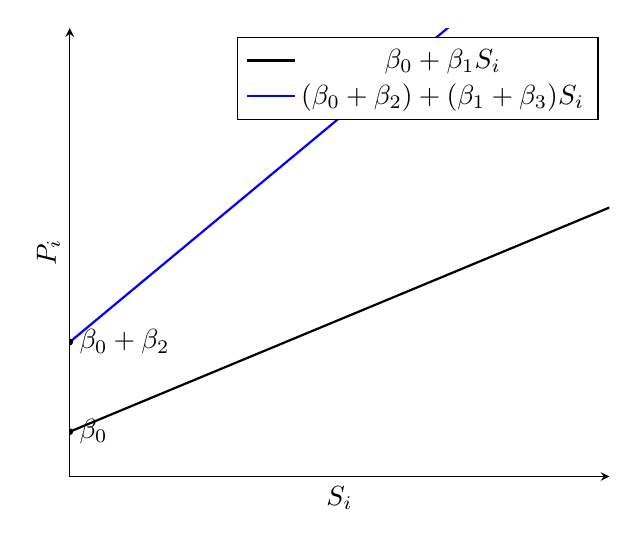
\begin{tikzpicture}
	\begin{axis}[axis lines = left, xmin = 0, ymin = 0, xmax = 10, ymax = 10, xlabel = $S_i$, ylabel = $P_i$, ticks=none]
		\addplot[domain=0:10,black, thick]{0.5 * x+1};
		\addlegendentry{$\beta_0+\beta_1 S_i$}
		\addplot[domain=0:10,blue, thick]{x+3};
		\addlegendentry{$(\beta_0+\beta_2)+(\beta_1+\beta_3) S_i$}
		\draw(axis cs:0,1)[fill]circle(1pt)node[right]{$\beta_0$};
		\draw(axis cs:0,3)[fill]circle(1pt)node[right]{$\beta_0+\beta_2$};
	\end{axis}
\end{tikzpicture}

\end{document}
